\section{Evaluation}\seclabel{Evaluation}
In this section, we describe Lucy: an implementation of our decision procedures
and system models. We then evaluate Lucy by answering the following questions:
\begin{itemize}
  \item
    How practical is the interactive invariant-confluence decision procedure?
    Can we use it to classify real-world transactions and invariants?
  \item
    How practical is segmented invariant-confluence? Are real-world workloads
    amenable to segmentation?
  \item
    How efficient is the interactive invariant-confluence decision procedure?
  \item
    How efficiently can we replicate a segmented invariant-confluent object as
    compared to alternative approaches like replicating with weak or strong
    consistency?
  \item
    How does the performance of replicating a segmented invariant-confluence
    object vary as we vary the workload, segmentation, and replication factor?
\end{itemize}

\subsection{Lucy}
Lucy includes an implementation of the interactive decision procedure described
in \algoref{InteractiveDecisionProcedure}, an implementation of a decision
procedure which checks criteria (1) - (4) from \thmref{LatticeProperty}, and an
implementation of the decision procedure described in
\algoref{ArbitraryStartInteractiveDecisionProcedure}. The decision procedures
are implemented in roughly 2,500 lines of Python. Users specify objects,
transactions, and invariants in a small Python DSL and interact with the
interactive decision procedures using an interactive Python console. We use
Z3~\cite{de2008z3} to implement our invariant-closure decision procedure,
compiling objects and invariants into a formula which is satisfiable if and
only if the object is \emph{not} invariant-confluent. If the object is
invariant-closed, then Z3 concludes that the formula is unsatisfiable.
Otherwise, if the object is not invariant-closed, then Z3 produces a
counterexample witnessing the satisfiability of the formula.

Lucy also includes an implementation of the invariant-confluence and
segmented-invariant confluence system models in roughly 3,500 lines of C++.
Users specify objects, transactions, invariants, and segmentations in C++. Lucy
then replicates the objects using invariant-confluence, segmented
invariant-confluence, eventual consistency, or linearizability. In
\secref{SegmentedInvariantConfluenceEval}, we compare the performance of these
various consistency models.
%
Because fault-tolerance is largely an orthogonal concern to
invariant-confluence, Lucy is implemented without fault-tolerance. It would be
straightforward to add fault-tolerance to Lucy, but it would not affect our
discussions or evaluation, so we leave it for future work. Moreover, users
currently have to specify their workloads in Python (for the decision
procedures) and C++ (for the runtime). In the future, we plan on removing this
redundancy.

\subsection{Decision Procedures}
% \todo{Bank account with and without decrements.}
% \todo{Auction example.}
% \todo{Foreign keys with and without deletions.}
% \subsection{TPC and Feral}
% \todo{See which of the Feral and TPC transactions we can determine automatically}

\subsection{Segmented Invariant Confluence}\seclabel{SegmentedInvariantConfluenceEval}
% \todo{one graph: number of locked operations x axis; throughput on the y-axis}
% \todo{one graph: number of segments on the x-axis; throughput on the y-axis}
% \todo{compare with no coordination and "VR"}

\begin{figure}[ht]
  \centering

  \begin{subfigure}[c]{\columnwidth}
    \centering
    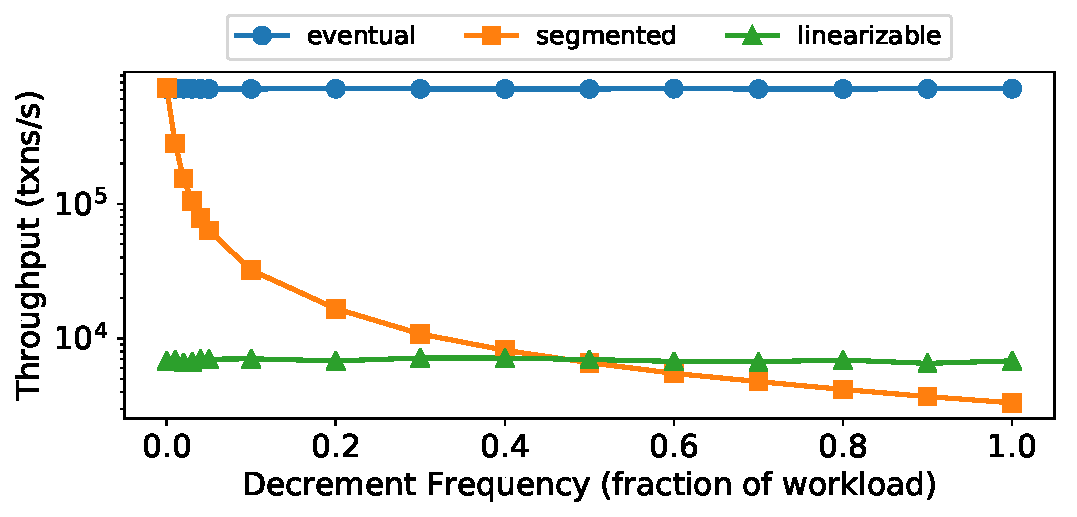
\includegraphics[width=\columnwidth]{figures/vary_withdraws.pdf}
  \end{subfigure}
  \begin{subfigure}[c]{\columnwidth}
    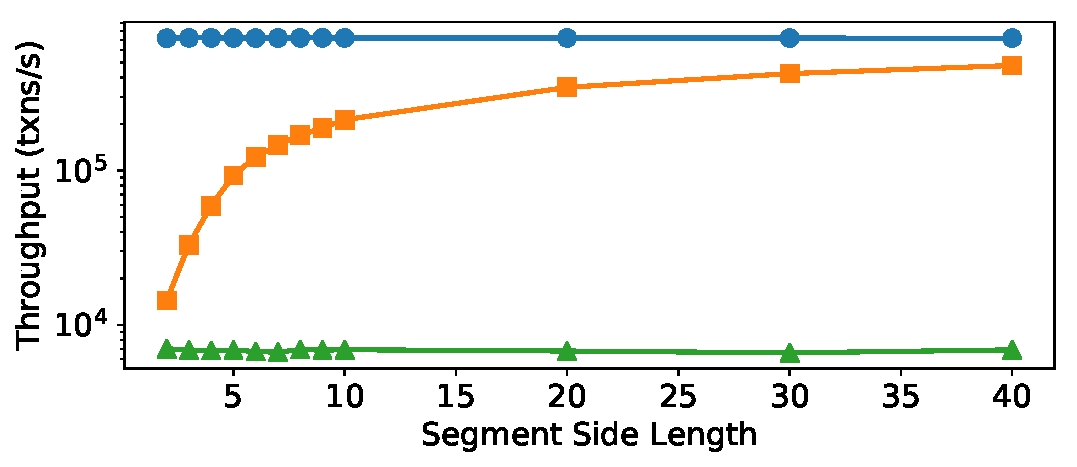
\includegraphics[width=\columnwidth]{figures/vary_segments.pdf}
  \end{subfigure}

  \caption{}\figlabel{}
\end{figure}

\begin{figure}[ht]
  \centering
  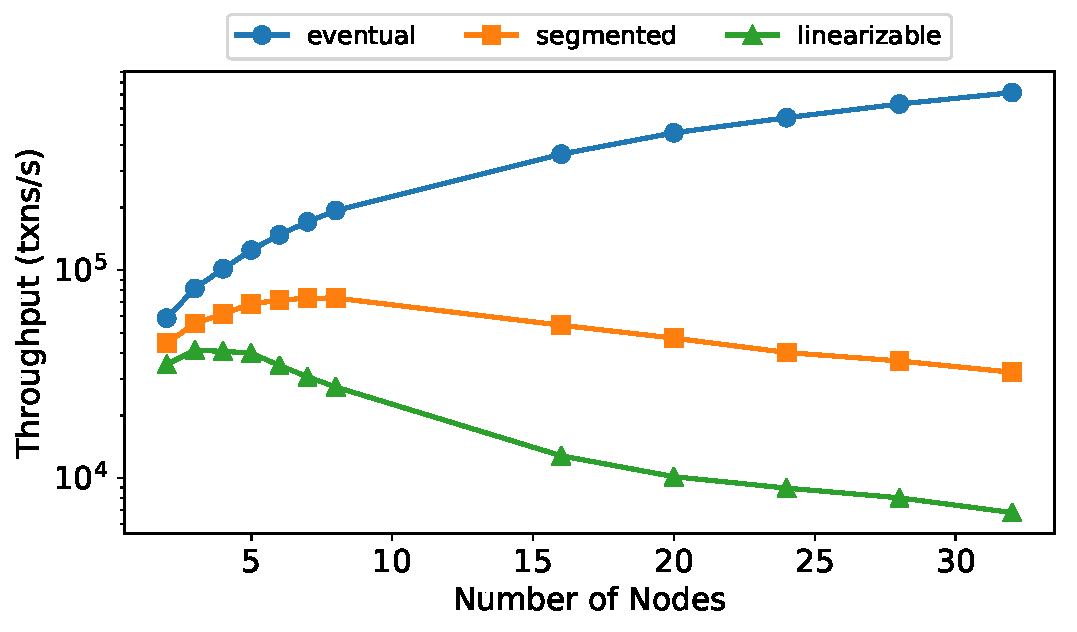
\includegraphics[width=\columnwidth]{figures/vary_nodes.pdf}
  \caption{}\figlabel{}
\end{figure}

\uselengthunit{in}\printlength{\columnwidth}
